% ---------
% --------
%!TEX TS-program = pdflatex
%!TEX encoding = UTF-8 Unicode
%!TEX spellcheck = English (Aspell)

\documentclass[11pt]{article}
\usepackage{lucy,handout,graphicx}
\usepackage{fourier-orns}
\usepackage{mathtools}
\usepackage[normalem]{ulem} % either use this (simple) or
\usepackage{tikz}
\usetikzlibrary{graphs}

\allowdisplaybreaks


\begin{document}

\noindent Name \underline{\hspace{12cm}}\\

\begin{center}
\Large\textbf{CSCI 332, Fall 2026}\\
\LARGE\textbf{Exam 2 Practice 1}
\end{center}

\noindent This exam consists of the following sections:
\begin{enumerate}
    \item Graph algorithms (35 points)
    \item Graph problems (40 points)
    \item P vs. NP (35 points)
\end{enumerate}

You may use a double sided 3x5 handwritten notecard of notes during the test but no other resources.

Good luck!

\newpage

\begin{center}
\LARGE\textbf{Section 1 (Graph algorithms)\\}%
\end{center}

\begin{enumerate}
    \item The following problems refer to the graph $G$ below. Ignore 
    edge weights in parts (a) and (b).
    \begin{center}
    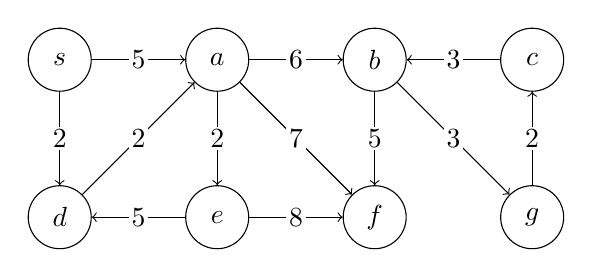
\begin{tikzpicture}[
        vertex/.style={circle,draw, minimum size = 8mm},
        edge/.style={->},
        label/.style={midway, fill=white, inner sep=1pt}
    ]
        \node[vertex] (s) at (0,2) {$s$};
        \node[vertex] (a) at (2,2) {$a$};
        \node[vertex] (b) at (4,2) {$b$};
        \node[vertex] (c) at (6,2) {$c$};
        \node[vertex] (d) at (0,0) {$d$};
        \node[vertex] (e) at (2,0) {$e$};
        \node[vertex] (f) at (4,0) {$f$};
        \node[vertex] (g) at (6,0) {$g$};

        \draw[edge] (s) -- node[label] {$5$} (a);
        \draw[edge] (a) -- node[label] {$6$} (b);
        \draw[edge] (c) -- node[label] {$3$} (b);
        \draw[edge] (s) -- node[label] {$2$} (d);
        \draw[edge] (d) -- node[label] {$2$} (a);
        \draw[edge] (a) -- node[label] {$2$} (e);
        \draw[edge] (a) -- node[label] {$7$} (f);
        \draw[edge] (b) -- node[label] {$5$} (f);
        \draw[edge] (b) -- node[label] {$3$} (g);
        \draw[edge] (g) -- node[label] {$2$} (c);
        \draw[edge] (e) -- node[label] {$5$} (d);
        \draw[edge] (e) -- node[label] {$8$} (f);
    \end{tikzpicture}
    \end{center}
    \begin{enumerate}
        \item List the strongly connected components of $G$.
        \vspace{1in}
        \item Draw the metagraph of $G$.
        \vspace{1in}
        \item For each node $v$, give $dist(s, v)$ (the shortest-path distance from $s$ to $v$).
        \begin{itemize}
            \item $dist(s, s) = $
            \item $dist(s, a) = $
            \item $dist(s, b) = $
            \item $dist(s, c) = $
            \item $dist(s, d) = $
            \item $dist(s, e) = $
            \item $dist(s, f) = $
            \item $dist(s, g) = $
        \end{itemize}
        \item Draw a shortest-path tree rooted at $s$ that is traced out by
        calls to whatever-first-search using a priority queue.
        If needed, break ties alphabetically.
    \end{enumerate}

    \newpage
    \item Recall the DFS algorithm that records pre and post order:
   \par\vspace{1em} 
    \begin{minipage}[t]{0.43\linewidth}
    \begin{algo}
    DFSAll($G$):\+\\
        $clock \gets 0$\\
        for all vertices $v$:\+\\
            unmark $v$\-\\
        for all vertices $v$:\+\\
            if $v$ is unmarked:\+\\
                $clock \gets \mathrm{DFS}(v, clock)$\-\-
    \end{algo}
    \end{minipage}\hfill
    \begin{minipage}[t]{0.54\linewidth}
    \begin{algo}
    DFS($v, clock$):\+\\
        mark $v$\\
        $clock \gets clock + 1$\\
        $v.\mathrm{pre} \gets clock$\\
        for all edges $v \to w$:\+\\
            if $w$ is unmarked:\+\\
                $w.\mathrm{parent} \gets v$\\
                $clock \gets \mathrm{DFS}(w, clock)$\-\-\\
        $clock \gets clock + 1$\\
        $v.\mathrm{post} \gets clock$\\
        return $clock$
    \end{algo}
    \end{minipage}
\par\vspace{1em}
Suppose this algorithm is run on some unknown graph with
the following
$v$.pre and $v$.post values assigned.
    \begin{center}
    \begin{tabular}{lrr}
        Vertex & Pre & Post \\
        \hline
        $A$ & 1 & 6 \\
        $B$ & 2 & 3 \\
        $C$ & 4 & 5 \\
        $D$ & 7 & 8 \\
    \end{tabular}
    \end{center}

    For each possible edge (listed below), circle whether it must exist,
    might exist, or cannot exist in the unknown graph.

    \begin{enumerate}
        \item $A \to B$ must exist $\cdot$ might exist $\cdot$ cannot exist
        \item $A \to C$ must exist $\cdot$ might exist $\cdot$ cannot exist
        \item $A \to D$ must exist $\cdot$ might exist $\cdot$ cannot exist
        \item $B \to A$ must exist $\cdot$ might exist $\cdot$ cannot exist
        \item $B \to C$ must exist $\cdot$ might exist $\cdot$ cannot exist
        \item $B \to D$ must exist $\cdot$ might exist $\cdot$ cannot exist
        \item $C \to A$ must exist $\cdot$ might exist $\cdot$ cannot exist
        \item $C \to B$ must exist $\cdot$ might exist $\cdot$ cannot exist
        \item $C \to D$ must exist $\cdot$ might exist $\cdot$ cannot exist
        \item $D \to A$ must exist $\cdot$ might exist $\cdot$ cannot exist
        \item $D \to B$ must exist $\cdot$ might exist $\cdot$ cannot exist
        \item $D \to C$ must exist $\cdot$ might exist $\cdot$ cannot exist
    \end{enumerate}

\newpage

\begin{center}
\LARGE\textbf{Section 2 (Graph problems)\\}%
\end{center}

\item Suppose you are given a directed graph $G$ with $n$ vertices and $m$ edges
in which every edge is colored either pink or yellow, and a vertex $s$, and you
want to find all vertices $v$ such that G has a walk from $s$ to $v$ whose edges
alternate colors (that is, any two consecutive edges of the walk must have
different colors). 

Reduce this problem
to a standard reachability problem on a new graph $G'$ and apply
whatever-first search (WFS) as a black box. (That is, you may not modify WFS at all.)
Your goal is an $O(n + m)$-time algorithm. \textbf{Answer the following to describe your algorithm.}
\begin{itemize}
    \setlength{\itemsep}{60pt}
\item What are the vertices of $G'$ in relation to $G$?  What does each vertex represent?
\item What are the edges of $G'$ in relation to $G$?  Are they directed or undirected?
\item If the vertices and/or edges have associated values, what are they?
\item What is the precise relationship between your graph $G'$ and the stated problem?
\item You must use WFS to solve the problem. What do you call it on, and how do you
interpret the result?
\item Describe and justify the running time of your entire algorithm,
\emph{including} the time to build $G'$, \emph{as a function of the original
input parameters}.
\end{itemize}

\newpage

\item To finish a video game, you must fight the final boss. But fighting the final
boss requires fighting a number of other bosses, and each of those bosses may have
other bosses that must be fought before them.
You are given the name of the final boss and a list of
pairs \((A,B)\), each meaning that fighting \(A\) requires fighting \(B\) first.

To solve this problem, you decide to build a graph where each node is a boss and
each edge points in the same direction as the ordered pairs.

\begin{enumerate}
    \item Draw the graph for the following input: Ash is the final boss, and
    pairs are (Ash, Bolt), (Ash, Claw), (Bolt, Dusk), (Bolt, Echo), (Claw,
    Echo), (Claw, Fang), (Dusk, Grim), (Fang, Hex).
    \vspace{2in}
    \item How can you use a standard graph algorithm on the created graph to find
    a possible order to fight the bosses, if one exists?
\end{enumerate}
\newpage
\begin{center}
\LARGE\textbf{Section 3 (P vs. NP)\\}%
\end{center}

\item
For each of the following statements, indicate whether it is True or False.
\textbf{Assume P $\neq$ NP.}

\begin{enumerate}[(a)]
    \item Every problem in NP is also in P. T or F
    \item Every problem in P is also in NP. T or F
    \item The set NP is the set of problems that cannot be solved in polynomial time. T or F
    \item If a problem $A$ is NP-Complete, then $A$ is in NP. T or F
    \item If a problem $A$ is NP-Complete, then $A$ is in P. T or F
    \item If a problem $A$ is in NP, then there exists a polynomial-time
    verification algorithm for yes instances of $A$. T or F
    \item If there is a polynomial-time reduction from problem $A$ to NP-hard problem $B$,
    then problem $A$ is NP-hard. T or F
    \item If there is a polynomial-time reduction from NP-hard problem $A$ to problem $B$,
    then problem $B$ is NP-hard. T or F

\end{enumerate}

\item The \textsc{Knapsack} problem is defined as follows:
Given a set of $n$ items, each with a weight and a value,
determine the maximum total value of items that can be placed in a knapsack
of weight capacity $W$.

\begin{enumerate}
    \item Suppose $n=5$, $W=6$, and the five items have the following weights and values. Give
    the \textbf{maximum total value of items that can be placed in the knapsack}.

    \begin{tabular}{lrr}
        Item & Weight & Value \\
        \hline
        A & 4 & 7 \\
        B & 3 & 5 \\
        C & 3 & 5 \\
        D & 2 & 2 \\
        E & 1 & 1 \\
    \end{tabular}

    \item Write a \emph{decision} version of \textsc{Knapsack}.
    \vspace{1in}
    \item Prove that your decision version of the \textsc{Knapsack} problem is in NP.
\end{enumerate}
\newpage

\item Recall the polynomial-time reduction from $k$-\textsc{Independent-Set} to
$k$-\textsc{Vertex-Cover}:
    \begin{algo}
    $k$-Independent-Set($G$ with $n$ nodes):\+\\
        let $k'=n - k$\\
        run $k'$-Vertex-Cover on $G$\\
        return result
    \end{algo}

For each of the following, circle true or false.

\begin{enumerate}
    \item If we know that $k$-\textsc{Independent-Set} is NP-hard, then the
    polynomial-time reduction from $k$-\textsc{Independent-Set} to
    $k$-\textsc{Vertex-Cover} shows that $k$-\textsc{Vertex-Cover} is NP-hard.

    True $\cdot$ False

    \item If we know that $k$-\textsc{Vertex-Cover} is NP-hard, then the
    polynomial-time reduction from $k$-\textsc{Independent-Set} to
    $k$-\textsc{Vertex-Cover} shows that $k$-\textsc{Independent-Set} is NP-hard.

    True $\cdot$ False
\end{enumerate}
\end{enumerate}
\end{document}
